\chapter{PUMA - der digitale Zettelkasten}
\label{ch:digitaleZettelkasten}
Das Akademische Publikationsmanagement\index{Akademische 
Publikationsmanagement} (PUMA) ist ein System zum Sammeln, Verwalten, Teilen 
und Entdecken von Lesezeichen und Publikationen.\newline
Es ist zu vergleichen mit einem riesigen digitalen 
Zettelkasten, der für alle möglichen Quellen und Medien einsetzbar ist. PUMA 
ermöglicht Struktur und Ordnung für gesammelte Publikationen. Gespeicherte 
Publikationen und Lesezeichen lassen sich schnell wieder finden. Gleichzeitig 
bietet PUMA Platz für Notizen und Anmerkungen sowie eine Zusammenarbeit mit 
anderen PUMA-Nutzern. 
Die Software steht lizenzfrei als Webanwendung zur Verfügung.
\newline 
PUMA ist so konzipiert, dass es als alleiniges Eingabeportal für bibliografische Metadaten dienen kann. Außerdem können zu Literatureinträgen Dokumente hochgeladen werden. \newline
Durch die Vielzahl an Exportformaten und Schnittstellen zu anderen Programmen müssen die Nutzer ihre Daten nur einmal pflegen und können sie in anderen Systemen nachnutzen. Die wiederholte manuelle Eingabe von Publikationslisten entfällt. So können Forscher ihre Publikationslisten direkt aus PUMA auf ihre Homepage laden.  
\section{Für wen ist dieses Buch?} 
\label{sec:fuerWen}
Dieses Buch richtet sich an die Angehörigen der Universität Stuttgart.
Die im Buch erklärten Beispiele basieren auf der PUMA-Installation der 
Universität. Diese Beispiele gelten in leicht abgewandelter 
Version für jede Institution, die PUMA installiert hat. 
\newline
Externe, die nicht der Universität Stuttgart angehören, können sich nicht bei 
dem hier vorgestellten PUMA anmelden. Für sie bietet sich die Nutzung 
von BibSonomy an. Da PUMA und BibSonomy über fast die gleichen Funktionen und 
Möglichkeiten verfügen, lassen sich die Beispiele aus dem Buch mit leichten 
Abweichungen auch auf BibSonomy übertragen.\newline
Besonders geeignet ist PUMA für
\begin{itemize}
\item Forschende, die ihre eigenen Publikationslisten verwalten.
\item Mitarbeitende, die Publikationslisten von Projekten, 
Instituten oder Fakultäten pflegen.
\item Studierende, die Material für Examensarbeiten verwalten 
möchten.
\item Autorinnen und Autoren, die ihre Veröffentlichungen der Unibibliografie 
melden möchten.
\item Studierende sowie Wissenschaftlerinnen und Wissenschaftler, 
die in Arbeitsgruppen Literatur teilen möchten.
\end{itemize}
\section{Typische Anwendungsbeispiele für PUMA}
\label{sec:typischeAnwendung}
PUMA ist für die Nutzung im akademischen Bereich entwickelt worden.
Es hilft bei Literaturrecherchen für eine Haus-, Bachelor- oder Masterarbeit, 
indem die recherchierte Literatur in PUMA gespeichert werden kann. Webseiten und 
Publikationen können mittels einer Schaltfläche (Bookmarklet) im Browser direkt 
in PUMA abspeichert werden. Am Ende der Arbeit hilft PUMA dabei, das 
Literaturverzeichnis zu erstellen. Bei der Erstellung des Verzeichnisses kann 
aus 7.500 Zitationsstilen der passende ausgewählt werden oder auch eine 
individuelle Anpassung per Citation Style Language (CSL) vorgenommen werden.
\newline 
Eigene Veröffentlichungen können mit Hilfe von PUMA gepflegt und  durch den Tag 
\enquote{myown} gekennzeichnet werden. Dies vereinfacht das Erstellen einer 
Publikationsliste der eigenen Veröffentlichungen. Mit Hilfe des 
OpenCMS-Plugins kann die Publikationsliste direkt zum Beispiel auf der eigenen 
Homepage veröffentlicht werden und ist so für alle sichtbar.
\newline 
Ein weiteres typisches Anwendungsfeld bilden Institutspublikationslisten. 
Durch Erstellen einer Gruppe in PUMA kann eine gemeinsame Sammlung von 
Publikationen angelegt werden. Mit Hilfe des Plugins 
\enquote{Publikationsliste (aus BibSonomy/PUMA)} \index{Plugin für 
OpenCMS} kann eine Publikationsliste aus dieser 
Sammlung erzeugt werden.

   
\section{Anmelden\index{Anmeldung} bei PUMA} 
\label{sec:anmeldenBeiPuma}
\begin{figure}[h!]
 \centering
 \fbox{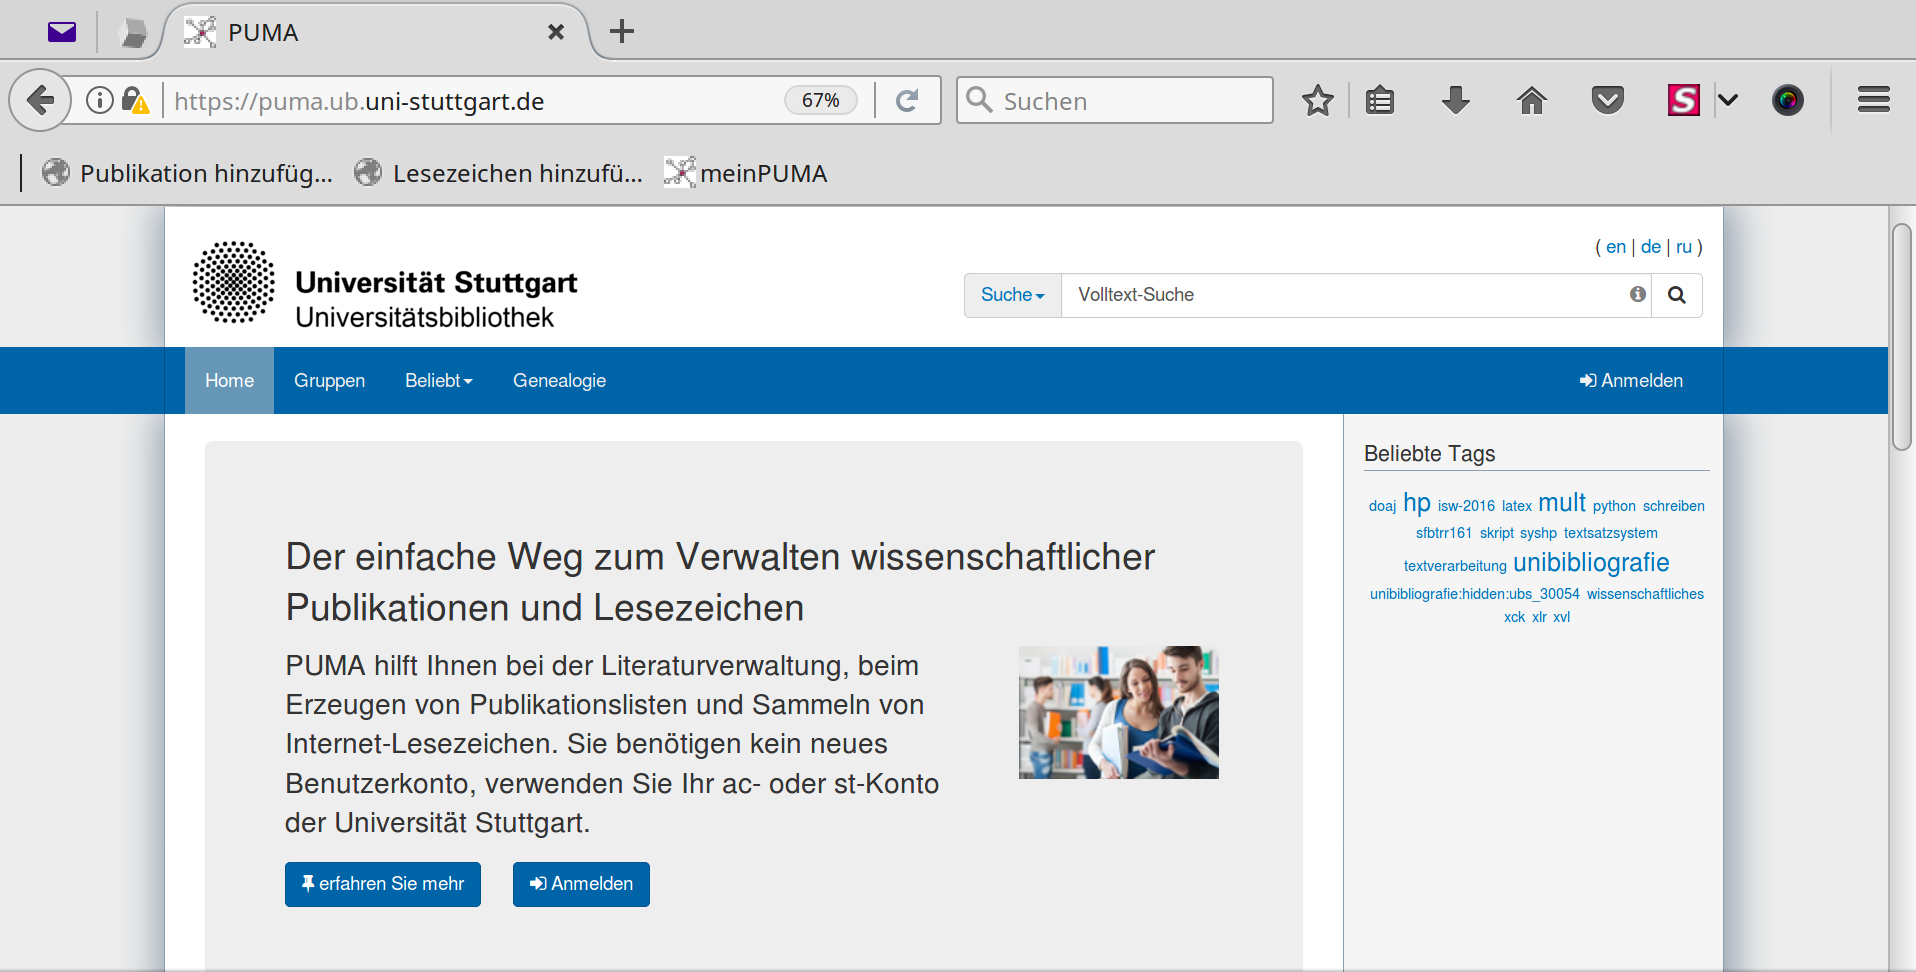
\includegraphics[width=10cm]{Bilder/Kapitel1/Startseite_PUMA}}
 \caption{Startseite PUMA}
 \label{fig:startseitePuma}
\end{figure}
\textbf{Vorab:} Es wird ein st-, fn- oder ac-Konto der Universität Stuttgart benötigt.
\begin{enumerate}
    \item Anmeldung über die PUMA-Homepage:\newline \url{https://puma.ub.uni-stuttgart.de/}
    \item Das ac- oder st-Konto der Universität Stuttgart und das Passwort eingeben (seltener ist ein fn-Konto).  
    \item Bei der Erstanmeldung muss ein selbstgewählter Benutzername vergeben werden.
\end{enumerate}
 \begin{figure}[h!]
 \centering
 \fbox{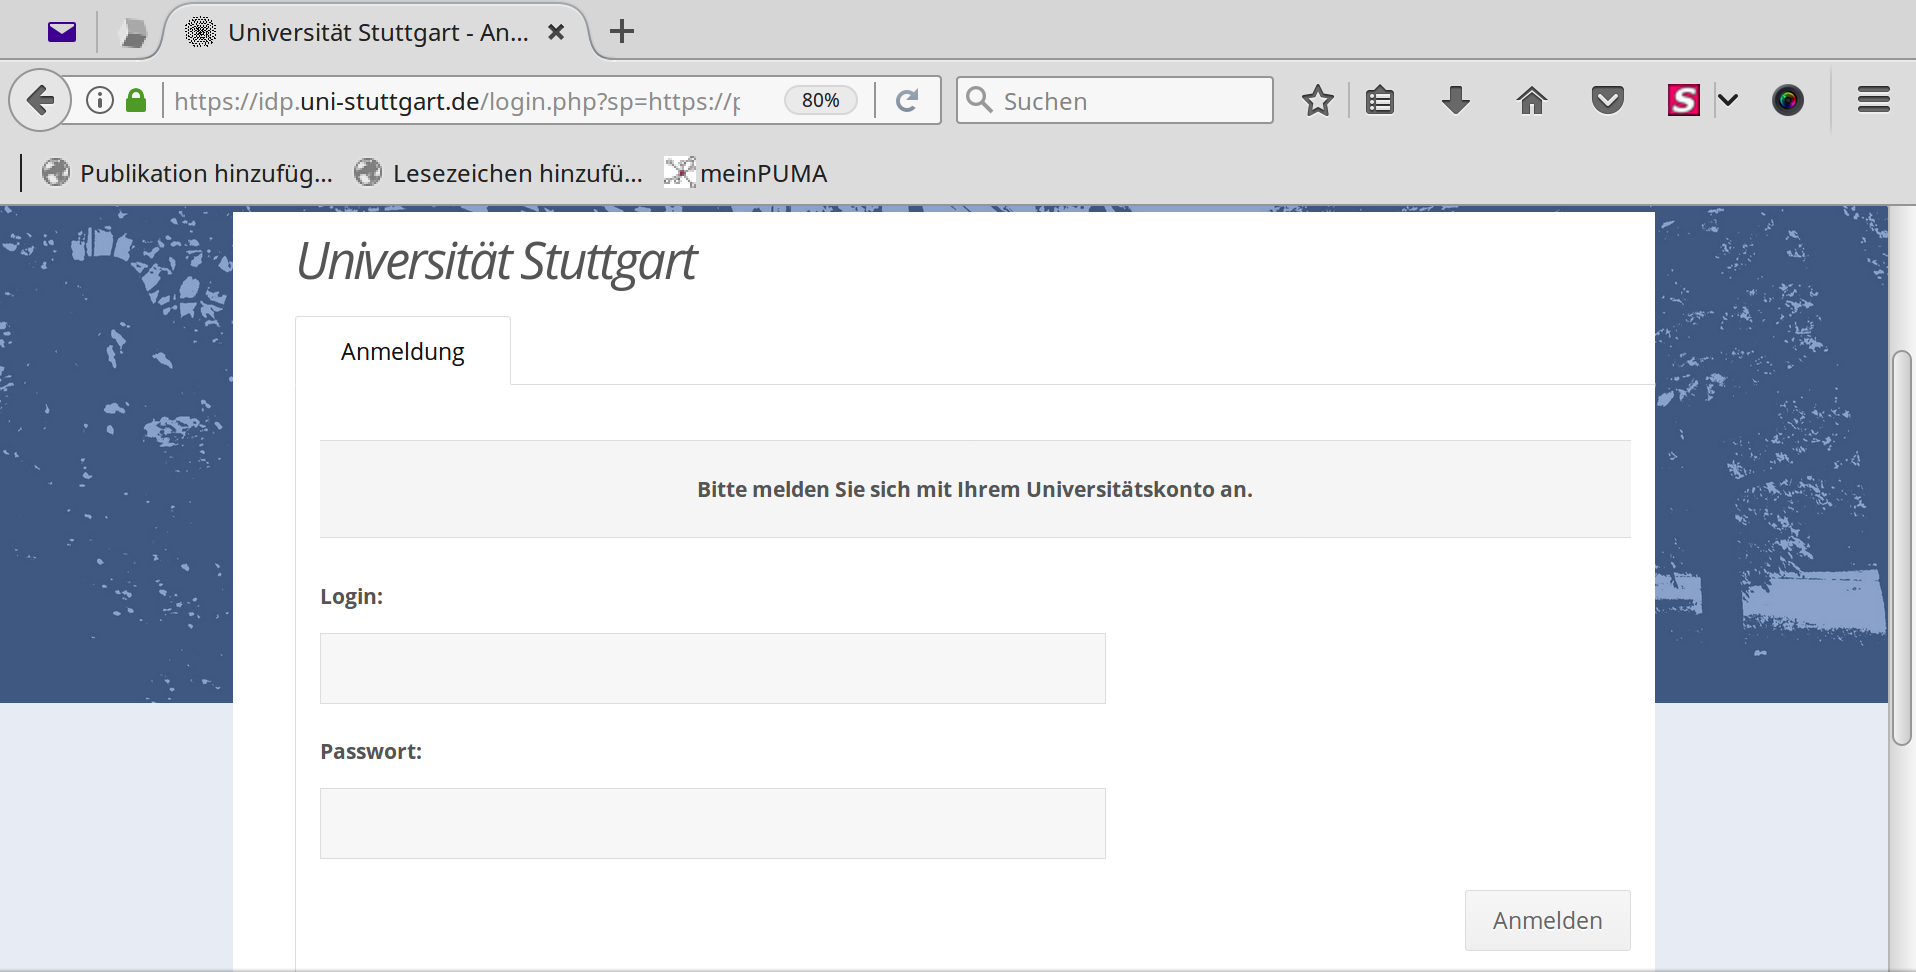
\includegraphics[width=9cm]{Bilder/Kapitel1/Anmeldung_bei_PUMA}}
 \caption{Anmeldung bei PUMA}
 \label{fig:anmeldungPuma}
\end{figure} 
Neben Publikationseinträgen ist der Benutzername öffentlich sichtbar (Grundeinstellung). Die Sichtbarkeit kann bei jedem Eintrag eingestellt werden. Der Benutzername wird mit einem vorangestellten \@-Zeichen dargestellt.
\section{Der PUMA-Blog}
\label{sec:pumaBlog}
Die Universitätsbibliothek Stuttgart (UB) informiert auf ihrem Blog über PUMA-Updates und neue Funktionen. Mit Hilfe eines RSS-Feeds können Interessierte die PUMA-Nachrichten abonnieren. Über den Link: \newline \url{http://blog.ub.uni-stuttgart.de/category/puma/feed/} werden die aktuellen Informationen angezeigt. \footnote{RSS ist ein einfaches Anzeigeformat für Internetnachrichten. Über \enquote{Jetzt abonnieren} auf der Blog-Seite der UB öffnet sich ein Fenster, in dem das Abonnieren nochmals bestätigt werden muss. Ab sofort können die Informationen über die Lesezeichen-Leiste im Browser angezeigt werden.}
 \begin{figure}[h!]
 \centering
 \fbox{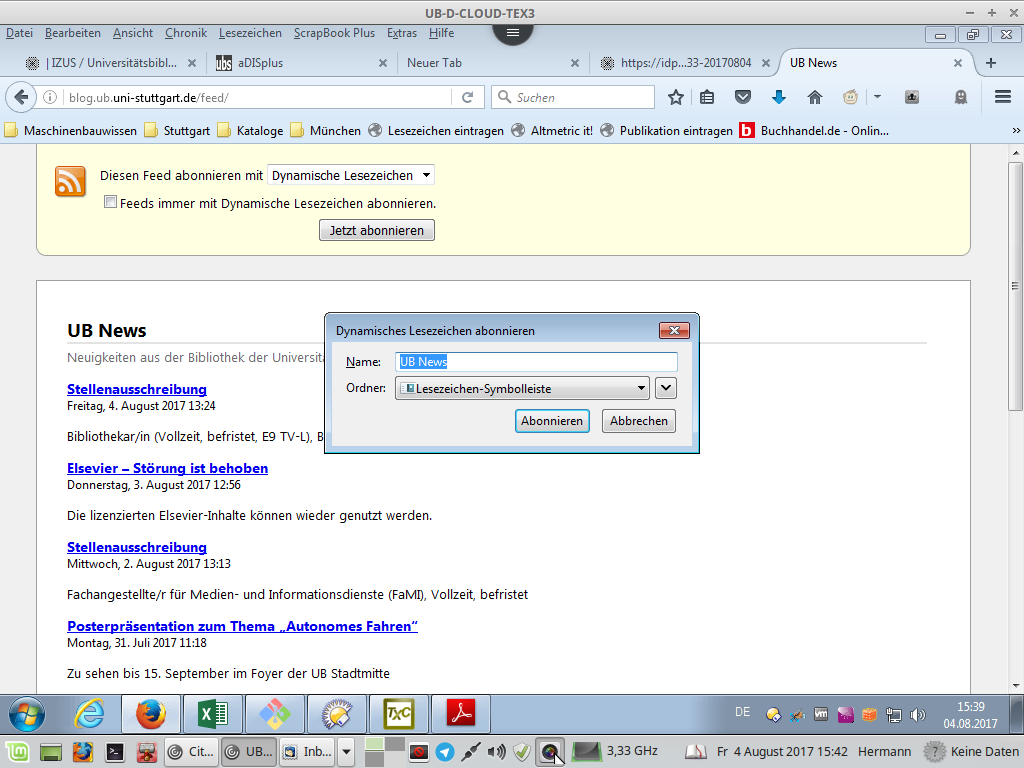
\includegraphics[width=9cm]{Bilder/Kapitel1/Anmeldung_Blog}}
 \caption{Anmeldung für RSS}
 \label{fig:anmeldungRss}
\end{figure} 
\section{BibSonomy\index{BibSonomy}}
\label{sec:bibsonomy}
BiBSonomy wurde von einem Team von Studierenden und Wissenschaftlern vom Fachgebiet Wissensverarbeitung der Universität Kassel entwickelt und bereitgestellt. In Zusammenarbeit mit der Universitätsbibliothek Kassel wurde die auf BibSonomy basierende Online-Literaturverwaltung PUMA entwickelt. Daher kann BiBSonomy weltweit nach einer Anmeldung \newline \url{http://www.bibsonomy.org/?lang=de} am System genutzt werden. Einträge aus PUMA können einfach nach BiBSonomy exportiert werden.

%\section{BibSonomy\index{BibSonomy} vs. PUMA}
%\suppressfloats[t]
\begin{table}[h!]
\tabulinesep=1.5mm
\begin{tabu}{|X[1.4,c]|X[2.2,m]|X[2,m]|} 
\tabucline[0.5pt]-\everyrow{\tabucline[0.5pt]-} 
\rowfont\bfseries
Unterschiede & PUMA \emph{Uni Stuttgart} & BibSonomy\\ \tabucline[1pt]-
\bfseries{Anmeldung}\strut & Nur möglich mit einem st-, fn- oder ac-Konto der Universität, mit dem sich die Nutzer authentifizieren.  & Für jeden frei zugänglich, ein Benutzerkonto muss selber angelegt werden. \\ 
\bfseries{Gruppen}\index{Gruppen} & Gruppen können jederzeit und selbständig gegründet werden. & Die Gründung einer Gruppe erfordert die Freigabe des BibSonomy-Admins. \\
\bfseries{OPUS}\index{OPUS} & Schnittstelle zu OPUS geplant. Ermöglicht den Nutzern ein direktes Veröffentlichen auf dem Dokumentenserver OPUS. & \\ 
\bfseries{Unibibliografie}\index{Unibibliografie}& Weiterverwendung von Metadaten aus der Unibibliografie möglich.&\everyrow{} \\ \tabucline[1.0pt]-
\end{tabu}
\caption{Unterschiede zwischen PUMA und BibSonomy}
\label{tab:unterschiedePumaBibsonomy}
\end{table}
%\normalsize